\documentclass[12pt,a4paper]{article}
\usepackage{ucs}
\usepackage{caption}
\usepackage[latin1,utf8x]{inputenc}
\usepackage{amsmath}
\usepackage{caption}
\captionsetup{font=small,labelfont=bf}
\usepackage[danish]{babel}
\usepackage[rmargin=3cm,tmargin=3.3cm]{geometry}
\usepackage{listings}
\usepackage{hyperref}
\setlength{\parindent}{0pt}
\setlength{\parskip}{1ex plus 0.5ex minus 0.2ex}
\usepackage{graphicx}
\usepackage{fixltx2e}

%insert links
\usepackage{hyperref}
\usepackage{fancyhdr,lastpage}	
\pagestyle{fancy}

%header
\lhead{ 
	Embedded Systems \\
	02131 \\ 
}
\chead{ 
}
\rhead{ 2 October, 2012 \\ \bigskip  }

%Footer
\lfoot{
	\rule{\textwidth}{0.1mm}\\
}

\cfoot{}
\rfoot{\ \\ \scriptsize{Side \thepage\ af \pageref{LastPage}}}

\begin{document}

%Forside
\begin{titlepage}
	\begin{center}
		\vspace*{13\baselineskip}
		\huge
		\bfseries
		Embedded Systems\\ 
		\ \\
		02131 \\[5\baselineskip]

		\normalfont
		\Large
		The ECG processor!\\	

		\small
		\vfill
	\end{center}	
	\begin{flushleft}
		Bastian Buch, s113432\\
	 	Jacob Gjerstruo, s113440\\
	\end{flushleft}
\end{titlepage}

\ \\
\section*{Abstract}
	The main task was implementing and integrating a dedicated hardware solution for the Moving Window Integration filter - a co-processor. By using Gezel, we have created the basic modules needed for the co-processor and have put these together into the actual co-processor. We have also begun testing that the co-processor works as intended. Our conclusion is that it is definitely feasible to create the hardware solution for the filter, and once done, it would be easy to compare the solution with an all-purpose-processor, and thus check the claims of a dedicated hardware solution being faster than an all-purpose processor.
\thispagestyle{empty} 
\newpage

%Table of Contents
\tableofcontents
\thispagestyle{empty} 
\newpage

%Reset pagecount
\setcounter{page}{1}

%Alm. sider
\ \\
\section{Introduction}
For this part, we have been hired by Medembed once again to investigate the benefits of implementing parts of the ECG scanner as a dedicated hardware implementation - in this case, we are to look into implementing a co-processor. For the purpose of this investigation, we have been tasked to implement a co-processor whose sole purpose will be to fulfil the calculations of the Moving Window Integration filter.
\section{Requirements}
For this assignment, we initially sat down and looked over the requirements, and in total, we found 5 functional requirements and one non-functional requirement. They are as follow: \\
\\
\textbf{ Functional requirements for the application:}
\begin{itemize}
	\item Integrating the processor with the rest of the system
	\item Identifying an algorithm for the co-processor
	\item Program the co-processor with the corresponding algorithm
	\item Integrate co-processor with the rest of the system
	\item An analysis of the implementation, including an analysis of speed, area and power
\end{itemize}
\textbf{Non-functional requirements for the application:}
\begin {itemize}
	\item The co-processor must be implemented in the Gezel language.
\end{itemize}

\newpage

\section{Analysis}
In designing the coprocessor, there were a few things we needed to consider:
\begin{enumerate}
	\item System integration
	\item How can a suitable algorithm for the processor be identified?
	\item How do we identify the needed functionality and determine the communication interface?
	\item How do we implement of the co-processor?
	\item How can the co-processor be integrated to the system?
	\item How can the performance be analysed?
\end{enumerate}

\subsection{Problem 1: Integrating the system}
	The first task of the assignment was to integrate the processor built in A2. As we unfortunately never managed to finish the processor in A2, we decided to skip this task and mainly focus on building the actual co-processor and, if we had time to spare, we would return and attempt to finish the processor and integrate it into the system.\\
	Unfortunately, we determined that we did not have time to spare for this task, and as such, we would only discuss the issues and solutions theoretically, rather than attempting to make the implementation of the processor and the integration of said processor ourselves.\\
	\\
	For doing this integration, we were given a very specific recipe on how it was to be made. When we were to connect the processor to the system, we would connect it to the BUS that uses a master/slave protocol, where the master would be the processor. When the processor is to communicate with the various components connected to it for data calculation, it would follow a simple protocol to ensure the data is parsed to the corresponding slaves (which can be seen on page 3 in Assignment 3: Implementation of an ECG co-processor \cite{lamport94}). The slave would then do the calculations and return the data through another similar protocol (which can be seen on page 5 in Assignment 3: Implementation of an ECG co-processor \cite{lamport94}).\\
	The challenges with this integration of the processor is to ensure a proper dataflow - that is, to ensure that the Master and the Slave actually communicates through the stated protocols. Once the dataflow between the Master and the Slave through the bus is correct, the integration of the processor would be complete.
\subsection{Problem 2: Identifying a suitable algorithm}
	When determining a suitable algorithm, it was necessary to consider three important aspects - high speed, low area and low power. We had to determine which of these were most important for us, and how we would accomplish the best ``performance'', in relation to what we see as being the most important of the three.
\subsection{Problem 3: Identifying the functionality and determining the communication interface}
	Having decided what the most important performance for us is, we needed to identify a suitable way to implement the operations needed to calculate the equation of the filter, which can be seen below.\\
	
	\begin{figure}[h!]
	  \centering
	    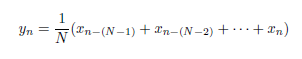
\includegraphics[width=0.5\textwidth]{Equation1.png}
	  \caption{The equation for the moving window integration filter}
	\end{figure}
	
	As can be seen on the equation, there are two ways the result can be calculated - one way is to divide each $x_n$ with 30, as N=30, and then sum it with the next division, and another would be to sum all the values of $x_n$ and then divide by 30. We were to determine which of these would be the best in terms of the performance we had chosen.\\
	Once this was done, we had to consider the communication interface, and determine how we would get the filter data from the memory to the co-processor, and how we would inform the co-processor to begin calculating. Thereafter, we were to find out how to get the data back out of the co-processor and find a way to stop the processor.

\subsection{Problem 4: Implementation of the co-processor}
	The next step would be to implement the co-processor. This would be done one step at a time - that is, first, we were tasked to design the components needed for the co-processor; then, we were to combine these components into the processor we needed in regards to the functionality, and test that this one works; and then we would have to add the communication interface and test that this works before and finally, before integrating the entire processor, we would have to test the entire system.
	Several challenges appeared during this task:
	\begin{enumerate}
		\item Which modules would be necessary?
		\item How many of each modules would be needed?
		\item How do we handle special cases - such as dividing with 0 or getting a negative input?
		\item What parts, specificly, needs to be tested?
	\end{enumerate}
\subsection{Problem 5: Integrating the co-processor into the system}
	Once the implementation of the co-processor would be done and we have tested that it works, we would have to integrate the co-processor with the rest of the system. This involves 3 subtasks - first, the co-processor must be connected to the bus via a slave interface. Secondly, a send command (SCMD instruction) had to be added to the all-purpose-CPU so we can send data to the co-processor, and finally, we had to write a small program to our processor which can communicate with our co-processor via the SEND COMMAND instruction.
\subsection{Problem 6: Analysing the performance}
When speaking of performance, there are three terms that needs to be discussed - size, speed and power. \\
The size of the coprocessor is important because the larger it is, the more power-consuming it will be, and secondly, as the ECG scanner in itself cannot be that large, there is a maximum size the processor can have. Furthermore, the larger the coprocessor is, the more modules is included and thus, more power is consumed.\\
The speed is of course also important - the coprocessor needs to be able to make a certain minimum number of calculations per second, in that the scanner itself, which will provide the coprocessor with data, will bring 250 data points to be calculated on per second, and it is important that the coprocessor is able to keep up with this stream of information, making the calculations and feeding them back to the main processor. On the other hand, it is also important that the coprocessor does not work too fast - having it consume lots of power to calculate, only to have it idle in-between data points would mean that energy is wasted, lowering the lifetime of the system itself.\\
Finally, power consumption is important in that the more energy the coprocessor consumes, the more often the battery on the scanner will need to be replaced or recharged - neither of which you want the costumer to bother with too often. The way to avoid this is either to reduce power consumption (by reducing the speed or the size) or to increase the battery size - the latter of which can only be done to a certain degree as the ECG scanner has a specific size.\\
\begin{enumerate}
\item How large would the coprocessor be, how can this be measured and can this size be reduced?
\item What is the energy consumption and what can be done to reduce consumption?
\item How fast is the coprocessor, compared to the all purpose processor, and how much idle time is there between data points? 
\end{enumerate}

\section{Design}
	When we were designing the co-processor, we started out with deciding what modules we needed for the co-processor. We came up with the following list of modules:\\
	\begin{enumerate}
		\item Counter
		\item Adder
		\item Bitshifter / Divider
		\item RAM module
	\end{enumerate}
	The modules themselves are quite easy to describe. The counter simply takes a registry and adds one to the registry, which is necessary to keep track of the amount of input data so far - have we reached the 30 data points or not? The adder adds two numbers together, which is needed to sum the numbers up. The bitshifter module takes all numbers and shifts them to the right - in our case, we use it to shift all numbers 9 places right, and we use it to carry out our division. We also use this as a workaround to dividing with zero and avoiding small amounts of remnants from division that would vanish, as we are doing integer division. Finally, we use a RAM module to keep a check on all input numbers to ensure we do not have to load again later on.\\
	\\
	Each of the modules, except for the divider were taken from A2 and as such, we had already tested that they worked and as such, we decided not to test them individually. Therefore, we proceeded to take all of these modules and stitched them together with the divider into a co-processor. At first, though, we had to design the dividing module.\\
	\\
	The biggest challenge we had was how we would do the actual division. We were given a hint that bitshifting might be a good idea, and after some help from a friend of ours, we found the formula (x*y)>>z, where x is the number to be divided with, z is the amount of bits shifted and y is a correctional number to ensure that you divide with approximately 30, and not the numbers of bit shifted (for instance, if z were 5, we would divide with 32 and not 30, but if you then multiply x with 1.066667, you would approximately divide with 30). We calculated y from the equation $y/q=1/30$, where q is the number corresponding the bitshift (bitshifting with 5 yields a q of 32, bitshifting with 9 yields a q of 512).\\ However, we quickly discovered another challenge which was that Gezel only does integer calculation, meaning that in our equation, (x*y) would be rounded to the lowest whole number. That meant we could not just bitshift with 5 and then multiply - we had to increase the amount of bitshifts to increase the accuracy of the approximation.\\
	\\
	We found that since we have no numbers above 10000 as input parameters, we would use this number as a guideline. Furthermore, $10000/30$ is approximately 333.33, meaning that our calculation should preferably yield 332 (due to approximation, we would never actually reach 333 unless we bitshifted and multiplied with very high numbers). After some experimentation, we found that bitshifting with 9 would yield a y of approximately 17, and thus, our final divider block ended up with a formula that were $x=((y*17)>>9)$. The final result with this formula is then $x=((10000*17)>>9=332)$, which we found to be acceptable.\\
	\\
	Once we had all these modules stiched together, we began creating a testbench to ensure that the co-processor were working as we wanted it to.
\section{Implementation}
\subsection{Integrating the system}
	As noted earlier, we never got around to finishing the processor in A2 and as such, we did not have anything to integrate here. However, if we had finished the processor, integrating the processor with the rest of the system seems fairly straightforward, thanks to the extensive recipe we were given on master/slave interfaces that went quite in debt on the communication between these two and how to implement it. We would therefore just follow this recipe as given to us on page 3 to 5 in Assignment 3: Implementation of an ECG co-processor \cite{lamport94}
\subsection{Identifying a suitable algorithm}
	When we were looking at the three types of performance, we quickly decided that of the three, area were the least important. The current processes needed to make processors can do so in such small sizes that we decided not to be overly much concerned with this - the only reason we still find it somewhat important is that the size is determined by the number of modules, and the more modules, the larger the power consumption.\\
	Secondly, power consumption would be the second most important in regards to performance as we deemed it more critical that the processors are able to keep up with the stream of information that is brought in by the ECG scanner, and display this information to the patient.\\
	Thirdly, we decided that speed is quite important, at least to the point where the co-processor must be able to do at least 250 calculations per second, since the heart-scanner runs with a frequency rate of 250 Hz, and thus brings 250 data points per second which need to be calculated on. Once this threshold is reached - 250 calculations per second, including the communication back and forth between co-processor and all-purpose-CPU - the critical speed would have been reached and it was important it did not do -much- more than this number of calculations, as it would then go on idle and consume power without doing anything, increasing the need of a larger battery. We will nevertheless be using speed as our critical performance.\\
\subsection{Identifying the functionality and determining the communication interface}
	In regards to identifying the functionality of the algorithm, we decided early on that we would sum up first and then divide the sum, rather than divide each incoming number and then sum it up. We decided to take this approach because it would mean we would always know the sum of the numbers we are dividing on, and as such, when we reach 30 data points and are to calculate on the 31'st data point, we can take the very first data point we got in and subtract it from the sum, and then add the 31'st to the sum and divide. This would give a lot less calculations than if we would have to calculate the sum of the 30 numbers every time before we divide it.\\
	In regards to the communication interface, it was actually specified in A3 how we were to create this interface - we would need to implement two in signals - a CMD signal and a data signal - as well as 2 out signals - another CMD signal and another data signal. The in CMD signal would be parsed by our co-processor, and this signal is supposed to tell the co-processor what to do. The in data signal would tell the co-processor where it is supposed to fetch the data. The out CMD signal would then report back to the all purpose CPU that the data has been calculated and passed, and the out data signal would specify what the data is.
\subsection{Implementation of the co-processor}
	When we were implementing the co-processor, we decided to start out with developing the modules needed for the co-processor. We decided that we needed a counter, an adder, a RAM module and a bitshifter module. Furthermore, we discovered that we needed several adders to ensure that the calculations could be carried out in a single clock cycle - in fact, we needed 1 counter, 1 adder and 1 ALU to ensure this could happen fast enough. Of the bitshifter module, we only needed a single module.\\
	\\
	Thanks to the bitshifter module, we would avoid the special case where dividing by 0 could happen. Furthermore, the only other special case we could think of was if the input parameters would be negative, and should this happen, there would be a serious error in that all data, after having passed the 4'th filter that comes just before the Moving Window Integration filter squares all data, thus making them positive.\\
	When we then came to decide what we needed to test, we quickly determined that it would not be necessary to test the components for themselves - we already did that when we were developing them in the previous assignment, A2, and as such, it only made sense to test the co-processor as a completed system.\\		
\subsection{Integrating the co-processor into the system}
	Due to time constraints, we never actually got to the point where we could integrate the co-processor with the rest of the system. Therefore, we never actually got around to looking at the issues related to this problem.
\subsection{Analysing the performance}
	We never got to actually analysing the performance, but doing so is a simple task. At first, we would look at the size of the co-processor. The simplest way to do so is to simply count the number of modules the co-processor - along with the registries and their bit-width. When we were to then optimize it, we would look into which registries we might not need, and which we could reduce in width without compromising the integrity of the co-processor.\\
	We would then take a look at the power consumption. There are generally three important terms to consider - Switching, which is power consumption because of active components; Short-circuit, which is when nMOS and pMOS transistors are on at the same time; and Static, which is power consumption because of inactive components. When we were to optimize, we would choose only to look at switching, as the amount of power needed goes up proportional with the activity - meaning that if the activity goes up a lot, the power consumption goes even higher.\\
	One measures the amount of switching by looking at the amount of toggles there is per clock cycle - that is, the amount of bits switching from 0 to 1 or the other way around. Finding out just how many bits switch is quite easy in Gezel - we would just need to toggle on operation profiling, which is two commands. This would then show us the amount of evaluations and toggles, and through this tool, we would be able to see where we would need to optimize, and where we would be fine.\\
	Furthermore, we would also take an extra look at all the modules the co-processor consists of and see if we could optimize these, or if any of them are dispensable.\\
	Finally, we would get to our most important term - speed. At first, we would take a look of the amount of clock cycles it would take to get through 250 data points on average. We would then calculate how much time one clock cycle would take on average. Once those two are calculated, we would see if we are within the needed speed (250 data points per second). If we are able to perform this amount of calculation, we would generally see if it is possible to relax a bit on the optimization - speedwise - and see if we could optimize more in regards to size - that is, decrease the size -and- the speed, as this would also lower power consumption. However, if we are not within the needed boundaries of 250 data point calculations per second, we would need to ensure that less clock cycles are used so the co-processor is able to keep up with the incoming data flow.

\section{Results}
	When we had the algorithm defined, we set out to drawing a block diagram of how we believed our final system with the co-processor would look. We ended up changing direction a few times, but below is the final block diagram of the co-processor, amended with the communication signals.\\
	\begin{figure}[h!]
	  \centering
	    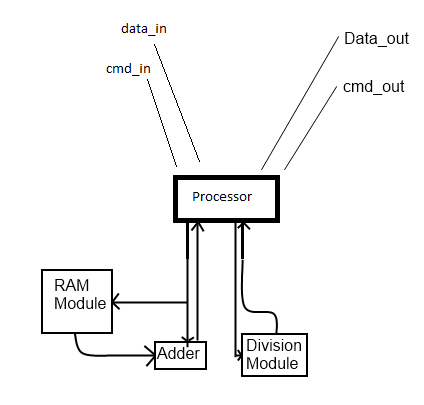
\includegraphics[width=0.75\textwidth]{Block_diagram2.png}
	  \caption{The amended block diagram with communication }
	\end{figure}
	\\
	Step one is, of course, that the processor receives a command signal that starts the calculation (cmd in), along with data to be calculated upon (data in). At this point, it saves the data in a ram block and then calculates the sum (beginning with 0+x, where x is the data that has just arrived). Once the data has been added to the sum, it is saved in a registry in the co-processor (here called Processor), which is then passed to the division module. This module divides the sum with 30, returns the result to the co-processor, and the co-processor then sends the data back to the all-purpose processor (data out), along with a signal (cmd out) that says ``All done now''.
\section{Conclusion}
	Due to time constraints, we were unable to integrate the processor from A2 and we were unable to analyse the performance of the co-processor we developed. We were, however, able to implement the necessary modules that had to be created for the co-processor, just as we were able to put the actual co-processor together. Finally, we started testing this co-processor but were unable to finish testing before time ran out.
\newpage
\begin{thebibliography}{9}

\bibitem{lamport94}
  Michael Reibel Boesen, Jan Madsen, Linas Kaminskas, Karsten Juul Frederiksen and Dusan Vuckovich\\
  \emph{Assignment 3: Implementation of an ECG co-processor}\\
  1st Edition\\
  2012.

\bibitem{Gezel Syntaks}
	Gezel Basic Syntaks pdf\\

\bibitem{Gezel user manual}
	\url{http://rijndael.ece.vt.edu/gezel2/manual.html} \\
	Date of use: 30/10-2012
	
\end{thebibliography}
	
\newpage	
	\begin{Large}
		\textbf{Appendix}
	\end{Large}
	\appendix

\section{Who wrote what}
Jacob Gjerstrup, s113440 wrote: Introduction, Requirements, Analysis, Design, Abstract, Conclusion\\
Bastian Buch, s113432 wrote: Requirements (50 percent), results\\
\\
For programming, a comment at each document has been made that shows whom programmed this particular part.
	
\section{Sourcecode}
\subsection{Co-processor}
	\lstinputlisting{Coprocessor_implementation.fdl}
\subsection{The individual modules}
	Here is a list of all the individual modules we used, alongside their testbench. They are:
	\begin{enumerate}
		\item Counter
		\item Adder
		\item Modified Adder
		\item RAM-block
		\item Division block
	\end{enumerate}	
	The sourcecode of these modules are listed below. The sourcecode for the modified adder has not been added as it is basicly just 
	
\subsubsection{Program Counter}
	\lstinputlisting{program_Counter.fdl}
\subsubsection{Adder}
	\lstinputlisting{program_Adder.fdl}
	\newpage
\subsubsection{RAM}
	\lstinputlisting{program_Instr_Mem.fdl}
\subsubsection{Divider}
	\lstinputlisting{program_divider.fdl}
\end{document}